\documentclass[10pt,a4paper]{article}
\usepackage[fontset=fandol,heading=true]{ctex}
\usepackage{fontspec,amsmath,amssymb,booktabs,tabularx,array,graphicx,xcolor}
\usepackage[left=19mm,right=19mm,top=17mm,bottom=18mm]{geometry}
\usepackage{caption,fancyhdr,microtype,needspace}
\usepackage[unicode,colorlinks=true,linkcolor=blue!45!black,urlcolor=blue!55!black]{hyperref}
\IfFontExistsTF{TeX Gyre Termes}{\setmainfont{TeX Gyre Termes}}{\setmainfont{Latin Modern Roman}}
\IfFontExistsTF{TeX Gyre Heros}{\setsansfont{TeX Gyre Heros}}{\setsansfont{Latin Modern Sans}}
\setmonofont{Latin Modern Mono}[Scale=.88]
\definecolor{ink}{HTML}{173348}
\definecolor{teal}{HTML}{217B70}
\definecolor{muted}{HTML}{556874}
\definecolor{light}{HTML}{EFF5F7}
\newcommand{\EN}[1]{\par\vspace{2pt}{\small\color{black!76}\noindent\textit{#1}\par}\vspace{4pt}}
\newcommand{\topic}[1]{\par\vspace{5pt}\noindent\textbf{#1}\quad}
\newcommand{\cost}{\mathcal C}
\newcommand{\dom}{\mathcal D}
\newcommand{\TPOT}{\mathrm{TPOT}}
\newcommand{\TTFT}{\mathrm{TTFT}}
\newcommand{\Pp}{\widehat P_P}
\newcommand{\Pd}{\widehat P_D}
\newcommand{\tp}{\widehat t_P}
\newcommand{\td}{\widehat t_D}
\newcommand{\interp}{\operatorname{lerp}}
\newcommand{\exPtime}{223.587}
\newcommand{\exPpower}{585.791}
\newcommand{\exPenergy}{130.975}
\newcommand{\exDtime}{11.704}
\newcommand{\exDpower}{603.479}
\newcommand{\exDenergy}{0.5886}
\newcommand{\exPmarginal}{212.022}
\newcommand{\exRate}{2.9686}
\newcommand{\exBusy}{0.6294}
\newcommand{\exQueue}{180.046}
\newcommand{\exMtpot}{31.581}
\newcommand{\exMttft}{435.214}
\newcommand{\exMpower}{592.346}
\newcommand{\exMenergy}{35.541}
\newcommand{\exPeObserved}{221.996}
\newcommand{\exPeError}{0.72}
\newcommand{\exDeContext}{2427.583}
\newcommand{\exDeObserved}{12.470}
\newcommand{\exDePredicted}{11.782}
\newcommand{\exDeError}{5.52}
\newcommand{\exEightLo}{1470.875}
\newcommand{\exEightHi}{4520.125}
\newcommand{\exEightPlo}{606.536}
\newcommand{\exEightPhi}{618.032}
\newcommand{\exEightWeight}{0.210257}
\newcommand{\exEightPower}{608.953}
\newcommand{\exSixteenLo}{1408.5625}
\newcommand{\exSixteenHi}{4453.0625}
\newcommand{\exSixteenPlo}{593.067}
\newcommand{\exSixteenPhi}{614.435}
\newcommand{\exSixteenWeight}{0.231052}
\newcommand{\exSixteenPower}{598.004}

\setlength{\parindent}{1em}
\setlength{\parskip}{2pt}
\linespread{1.05}
\setlength{\headheight}{14pt}
\setlength{\abovedisplayskip}{6pt}
\setlength{\belowdisplayskip}{6pt}
\renewcommand{\arraystretch}{1.18}
\captionsetup{font=small,labelfont=bf,skip=4pt}
\ctexset{subsection={format=\large\bfseries\color{ink},beforeskip=9pt,afterskip=4pt}}
\pagestyle{fancy}
\fancyhf{}
\fancyhead[L]{\small\sffamily PDblend\quad /\quad Offline profiling}
\fancyhead[R]{\small\sffamily Method note · 2026-09-24}
\fancyfoot[L]{\footnotesize\color{muted}Current implementation · Bilingual manuscript}
\fancyfoot[R]{\small\thepage}
\renewcommand{\headrulewidth}{.3pt}
\emergencystretch=1.5em
\hypersetup{pdftitle={PDblend Profiler: Formal Models and a Measured-Profile Example},pdfauthor={PDblend},pdfsubject={Bilingual profiler methodology with reproducible numerical examples}}
\begin{document}
\thispagestyle{empty}
{\LARGE\bfseries\color{ink}PDblend：离线性能与能耗建模}\par
\vspace{3pt}
{\large\sffamily Offline Performance and Energy Profiling}\par
\vspace{5pt}
{\small\color{muted}固定配置下的负载相关成本模型、验证流程与可复算实例\quad |\quad 2026-09-24}
\setcounter{secnumdepth}{2}
\setcounter{section}{0}
\renewcommand{\thesubsection}{\arabic{subsection}}

\subsection{Motivation}
稠密 Transformer 反复执行 QKV 投影、attention 和 MLP。QKV 与 MLP 以稠密线性运算为主，attention 还涉及 softmax 和 KV cache 访存。固定模型、TP、频率及执行环境后，计算和访存规模主要由请求形状决定，因而服务时间具有可建模的规律性。结合相同运行点下重复测得的窗口平均功率，可以进一步预测能量；这种可预测性需要测量验证，并不意味着耗时或功率恒定。
\EN{Dense Transformers repeatedly execute QKV projections, attention, and MLPs. QKV and MLP computations mainly involve dense linear operations; attention additionally involves softmax and KV-cache accesses. With the model, TP, frequency, and execution environment fixed, workload shapes largely determine computation and memory-access volumes. This regularity enables empirical service-time models and, together with repeatedly measured window-average power, energy prediction. Predictability requires measurement validation; it does not imply constant time or power.}

\subsection{Challenge}
当前 planner 联合枚举角色数量、分流阈值和频率。候选改变各池负载、排队及阶段干扰，逐个实际执行或在线进行细粒度性能分析代价高。Profiler 因此需要提供廉价的成本预测和明确的覆盖、容量边界，帮助筛除不可行候选。它降低候选评估开销，而不消除组合搜索。
\EN{The current planner enumerates role counts, routing thresholds, and frequencies. These choices change pool load, queueing, and phase interference. Executing every candidate or modeling its operators online would be expensive. The profiler supplies inexpensive estimates and explicit coverage and capacity boundaries to filter infeasible candidates. It reduces evaluation overhead without eliminating combinatorial search.}

\subsection{Insight}
将可复用的阶段成本与在线部署决策分离。固定配置后，以少量形状变量查询 prefill/decode 时间和功率；Mixed 由这些基础模型与负载、干扰模型组合。离线冻结的参数和表格可服务多个候选，planner 再统一计算时延与规划窗口能量。
\EN{Separate reusable phase costs from online deployment decisions. For each fixed configuration, a few shape variables determine prefill/decode time and power queries. Mixed execution combines these models with load and interference estimates. Frozen parameters and tables serve multiple candidates; the planner then derives latency and energy over a common planning horizon.}

\begin{center}
\begin{minipage}{\linewidth}
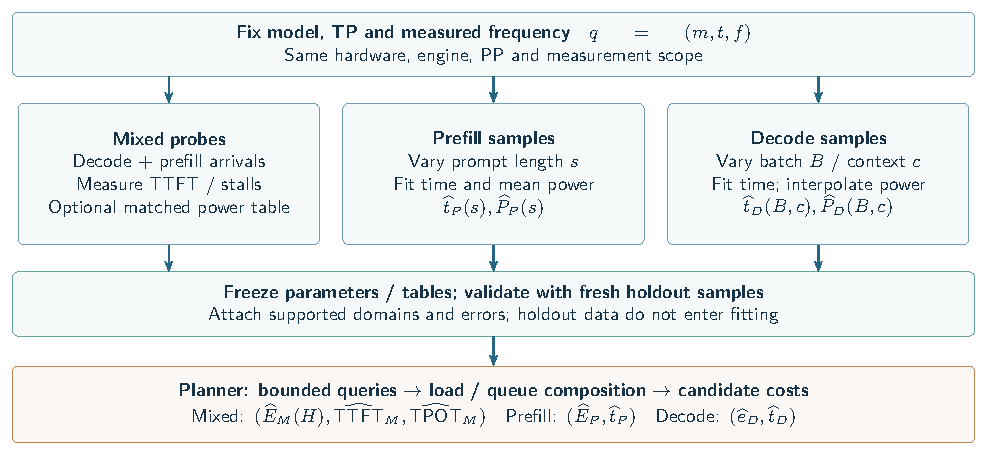
\includegraphics[width=\linewidth]{build/profiler-process.pdf}
\captionof{figure}{Profiler 的采样、建模、独立验证与查询过程。Mixed 由阶段模型组合；探针检查干扰，可选补测提供局部功率表。\\\textit{Profiling, modeling, independent validation, and queries. Mixed uses phase-model composition; probes check interference and optional panels supply local power tables.}}
\label{fig:process}
\end{minipage}
\end{center}

\newpage
\subsection{Approach}
固定硬件、引擎版本和 PP 后，以 $q=(m,t,f)$ 标识模型、TP 度和已测 GPU 频率。以下省略 $q$ 下标。$s$ 为输入长度，$B$ 为 decode batch，$c$ 为有效上下文，$N$ 为实例数，$H$ 为规划时长。功率均为\textbf{单个实例的 TP GPU 组总功率}，除非明确乘以 $N$。
\EN{Fix hardware, engine version, and PP, and index models by $q=(m,t,f)$: model, TP degree, and measured GPU frequency. We omit $q$ below. Let $s$ be prompt length, $B$ decode batch, $c$ effective context, $N$ instance count, and $H$ the planning horizon. Power denotes the total of one instance's TP GPU group unless explicitly multiplied by $N$.}

\begin{equation}
\begin{aligned}
\cost_M(F,N,H;q)&=(\widehat E_M(H),\widehat{\TTFT}_M,\widehat{\TPOT}_M),\\
\cost_P(s;q)&=(\widehat E_P(s),\tp(s)),\qquad
\cost_D(B,c;q)=(\widehat e_D(B,c),\td(B,c)).
\end{aligned}\label{eq:contract}
\end{equation}
这里 $F$ 包含到达率、长度统计和在途状态；$E_M,E_P$ 的单位为 J，$e_D$ 为 J/token，时间为 s。式~\eqref{eq:contract} 是组合后的成本接口；原始查询主要返回时间和功率。端到端排队与配置切换仍由 planner 处理。
\EN{$F$ includes rates, length statistics, and in-flight state. $E_M$ and $E_P$ use joules; $e_D$ uses J/token and times use seconds. Equation~\eqref{eq:contract} denotes the composed cost interface; primitive queries mainly return time and power. Queueing and configuration transitions remain planner responsibilities.}

\topic{Mixed：阶段组合 / Phase composition}
输入为 $F,N,H$；由负载推得 $B,c$。令 $\lambda_P$ 为池总等效 prefill 到达率，$\bar s,s_{95}$ 为平均及 95 分位输入长度。基础模型采用去除截距的边际 prefill 时间，估计其占用比例：
\EN{Given $F,N,H$, the planner derives $B,c$. Let $\lambda_P$ be the pool-wide effective prefill rate and $\bar s,s_{95}$ the mean and 95th-percentile prompt lengths. The base model removes the prefill intercept to estimate marginal work and its time fraction:}
\begin{equation}
\Delta\tp(s)=\max(a_1s+a_2s^2,0),\qquad
u_P=\frac{\lambda_P\Delta\tp(\bar s)}{N}<\rho_{\max}<1.
\label{eq:busy}
\end{equation}
\begin{equation}
\begin{aligned}
\widehat{\TPOT}_M&=\frac{\td(B,c)}{1-u_P},&
\widehat{\TTFT}_M&=W+\tp(s_{95})+\widehat{\TPOT}_M,\\
\widehat P_M&=N\bigl[u_P\Pp(\bar s)+(1-u_P)\Pd(B,c)\bigr],&
\widehat E_M(H)&=H\widehat P_M.
\end{aligned}\label{eq:mixed}
\end{equation}
$W$ 包含排队和 backlog 等待；上述 TTFT 为规划近似，并非严格尾分位保证。式~\eqref{eq:mixed} 写出活跃 $B\geq1$ 情况，低占用另按空闲占空比处理。Mixed 探针验证干扰近似，并不独立拟合整套成本。若存在匹配 batch、频率、prefill 长度与到达率的实测 Mixed 功率组件，则以其上下文插值替换组合功率。
\EN{$W$ includes queueing and backlog delay; TTFT is a planning approximation, not a strict tail-quantile guarantee. Equation~\eqref{eq:mixed} covers active $B\geq1$; lower occupancy uses a separate idle-duty treatment. Mixed probes check interference rather than fit a complete independent cost model. Where an optional measured Mixed-power component matches batch, frequency, prefill length, and arrival rate, its context interpolation replaces the composed power.}

\topic{Prefill：长度回归 / Length regression}
输入为 $s$，输出首 token 服务时间、平均功率及能量近似。时间采用二次回归；基础功率采用饱和仿射回归，当前 $s_{\rm sat}=1024$。查询计算拟合函数，无需查表插值：
\EN{The input is $s$; outputs are first-token service time, mean power, and approximate energy. Time uses quadratic regression; base power uses saturated affine regression with $s_{\rm sat}=1024$. Queries evaluate fitted functions rather than interpolate a table:}
\begin{equation}
\tp(s)=a_0+a_1s+a_2s^2,\quad
\Pp(s)=p_0+p_1\frac{\min(s,s_{\rm sat})}{s_{\rm sat}},\quad
\widehat E_P(s)=\tp(s)\Pp(s).
\label{eq:prefill}
\end{equation}
这里 $\tp$ 不含外部排队，$\widehat E_P$ 为服务口径的模型估计，不是单次请求能量积分；不能将该窗口功率与纯 CUDA kernel 时长混乘。
\EN{$\tp$ excludes external queueing. $\widehat E_P$ is a service-level model estimate, not a directly integrated single-request energy measurement. The window power must not be multiplied by a kernel-only CUDA duration.}

\newpage
\topic{Decode：时间拟合与功率插值 / Timing regression and power interpolation}
输入为 $B$ 与实际有效上下文 $c$，输出为稳态步长和组功率，再归一化为每 token 能量。短域校准将 $B=1$ 与 $B\geq4$ 分开回归；归一化常数吸收入系数后可写为：
\EN{Inputs are $B$ and actual effective context $c$. The model returns steady-state step time and group power, then normalizes energy per token. Short-domain calibration fits $B=1$ separately from $B\geq4$. Absorbing input-normalization constants into the coefficients gives:}
\begin{equation}
g_1(c)=d_0+d_1c,\qquad
g_h(B,c)=\alpha_0+\alpha_1B+\alpha_2Bc+\alpha_3B^2,
\label{eq:decodebase}
\end{equation}
\begin{equation}
\td(B,c)=\begin{cases}
g_1(c), & B=1,\\
g_1(c)+\dfrac{B-1}{3}\bigl[g_h(4,c)-g_1(c)\bigr], & 1<B<4,\\
g_h(B,c), & B\geq4.
\end{cases}\label{eq:decode}
\end{equation}
因此，主要时间模型由回归获得，$1<B<4$ 的时间连接段使用线性插值；它不自动授予同区域的功率覆盖。校准时间参数最小化训练样本的相对平方误差；基础功率回归则使用普通最小二乘。
\EN{Thus, timing is primarily regressed, with a linear bridge for $1<B<4$; this bridge does not grant power coverage in that regime. Calibrated timing parameters minimize squared relative training error, while the base power regression uses ordinary least squares.}
\begin{equation}
\theta^*=\arg\min_\theta\sum_{i\in\mathcal T}
\left(\frac{\widehat t_\theta(x_i)-t_i}{t_i}\right)^2.
\label{eq:fit}
\end{equation}

\topic{什么时候插值 / Where interpolation applies}
校准 Decode 功率表为每个实测 batch 保存有效上下文区间及窗口平均功率。区间内使用该均值；相邻区间之间沿 $c$ 插值。精确 batch 直接查询对应曲线；仅当 $4\leq B_0<B<B_1$ 时，在相邻实测 batch 间插值。定义 $\interp(z;z_0,z_1,v_0,v_1)$，则
\EN{For each measured batch, calibrated power tables store context bands and window-average power. Use the mean within a band and interpolate along $c$ between bands. Exact batches query their own curve; interpolate between neighboring measured batches only for $4\leq B_0<B<B_1$. Defining $\interp$ gives:}
\begin{equation}
\begin{aligned}
\interp(z;z_0,z_1,v_0,v_1)
&=v_0+\frac{z-z_0}{z_1-z_0}(v_1-v_0),\\
\Pd(B,c)&=\interp\bigl(B;B_0,B_1,\Pd(B_0,c),\Pd(B_1,c)\bigr),\\
\widehat{\TPOT}_D&=\td(B,c),\qquad
\widehat e_D(B,c)=\frac{\td(B,c)\Pd(B,c)}{B}.
\end{aligned}\label{eq:interp}
\end{equation}
$B=1$ 的功率单独处理；可选 $B=2,3$ 组件要求精确 batch 匹配。长上下文扩展固定实测 batch 和频率，时间与功率均沿上下文分段插值。所有插值均受覆盖域限制，不跨频率或未覆盖域外推。由于功率已对 TP 组求和，能量不再乘 TP。
\EN{Power at $B=1$ is separate; optional $B=2,3$ components require exact batches. Long-context extensions fix measured batch and frequency and interpolate both time and power along context. All interpolation is bounded by coverage, with no interpolation across frequencies or extrapolation into unsupported domains. Power already sums the TP group, so energy is not multiplied by TP again.}

\topic{从测量到可查询模型 / From measurements to queryable models}
Prefill 使用预热后的重复单请求。Decode 等全部请求完成 prefill 并继续推进后，在持续生成中稳定至少 2 秒，再测量至少 5 秒，每点至少三个窗口；记录实际 token 进度、功率和频率。拟合或建表后冻结参数，用独立留出样本评估误差；发布时同时保存身份与覆盖域。
\EN{Prefill uses warmed-up repeated single requests. Decode waits until all requests finish prefill and advance further, settles for at least two seconds under continuous generation, and measures for at least five seconds, with at least three windows per point. Actual token progress, power, and clocks are recorded. Parameters are frozen after fitting or table construction and evaluated on independent holdouts; publication preserves identity and coverage.}
\begin{equation}
\epsilon_i=\frac{|\widehat y_i-y_i|}{|y_i|},\qquad
\dom_q=\dom_{\rm time}\cap\dom_{\rm power}\cap\dom_{\rm KV}.
\label{eq:valid}
\end{equation}
训练残差不能替代留出误差；覆盖之外返回缺测，而非零成本。训练、校准、Mixed 组合与整机能量验证是不同层次。
\EN{Training residuals do not replace holdout errors. Queries outside coverage report missing measurements, not zero cost. Training, calibration, Mixed composition, and full-system energy validation are distinct stages.}

\newpage
\topic{具体例子 / Worked example}
选择已有校准组件：Qwen2.5-7B-Instruct，TP4、PP1、2100 MHz，四张 L20 的组功率。下列数字由冻结系数与功率表复算；$s=2048,B=12,c=2112$ 是域内查询条件，\textbf{不是声称在该点新做了 GPU 实验}。
\EN{Use an existing Qwen2.5-7B-Instruct component at TP4, PP1, 2100 MHz, with power summed over four L20 GPUs. The numbers below are recomputed from frozen coefficients and power tables. $s=2048,B=12,c=2112$ defines an in-domain query, not a newly executed GPU experiment.}

\begin{center}\small
\begin{tabular}{@{}lrrr@{}}
\toprule
查询 / Query & 时间 / Time & 功率 / Power & 能量估计 / Energy estimate\\
\midrule
Prefill: $s=2048$ & \exPtime\ ms & \exPpower\ W & \exPenergy\ J/prefill\\
Decode: $B=12,c=2112$ & \exDtime\ ms/step & \exDpower\ W & \exDenergy\ J/token\\
\bottomrule
\end{tabular}
\end{center}

\topic{1. 拟合查询 / Regression query}
在该频率，$a_0=0.0115648275$，$a_1=1.01305325\times10^{-4}$，$a_2=1.08448023\times10^{-9}$。代入式~\eqref{eq:prefill} 得 $\tp(2048)=\exPtime$ ms。Decode 将 $B,c$ 代入式~\eqref{eq:decodebase}，得到 $\exDtime$ ms；这一步不使用功率表。
\EN{At this frequency, substituting the listed prefill coefficients into Eq.~\eqref{eq:prefill} yields $\exPtime$ ms. Evaluating the decode regression at $B,c$ yields $\exDtime$ ms; timing does not query the power table.}

\topic{2. 两级插值 / Two-stage interpolation}
训练功率表在 $B=8,16$ 的相邻上下文区间之间提供以下端点；端点取低区间上界和高区间下界。
\EN{The training power table supplies these endpoints between neighboring context bands at $B=8,16$: the upper edge of the lower band and lower edge of the upper band.}
\begin{center}\small
\begin{tabular}{@{}rrrrrr@{}}
\toprule
$B$ & $c_0$ & $c_1$ & $P_0$ (W) & $P_1$ (W) & $\Pd(B,2112)$ (W)\\
\midrule
8 & \exEightLo & \exEightHi & \exEightPlo & \exEightPhi & \exEightPower\\
16 & \exSixteenLo & \exSixteenHi & \exSixteenPlo & \exSixteenPhi & \exSixteenPower\\
\bottomrule
\end{tabular}
\end{center}
\begin{equation}
\begin{aligned}
\Pd(12,2112)&=\tfrac12(\exEightPower+\exSixteenPower)
\simeq\exDpower\ \mathrm W,\\
\widehat e_D&=\frac{(\exDtime\times10^{-3})\times\exDpower}{12}
\simeq\exDenergy\ \mathrm{J/token}.
\end{aligned}\label{eq:example}
\end{equation}

\topic{3. 独立测量对照 / Independent timing observations}
以下使用已有留出样本的汇总值，Decode 使用实际有效上下文。这里检验时间预测，不把示例能量标成实测。
\EN{The following comparisons use existing holdout summaries and actual effective decode context. They check timing predictions, not measured example energy.}
\begin{center}\small
\begin{tabular}{@{}lrrr@{}}
\toprule
留出条件 / Holdout shape & 实测 / Observed & 预测 / Predicted & 相对误差 / Error\\
\midrule
Prefill $s=2048$ & \exPeObserved\ ms & \exPtime\ ms & \exPeError\%\\
Decode $B=12,c=\exDeContext$ & \exDeObserved\ ms & \exDePredicted\ ms & \exDeError\%\\
\bottomrule
\end{tabular}
\end{center}

\topic{4. Mixed 组合 / Mixed composition}
构造无 backlog 的单实例负载：输入 2048、平均输出 128 tokens，$\lambda_P=\lambda_D=\exRate$ req/s，$H=60$ s。此时 $c=2048+128/2=2112$，$u_P=\exBusy$，并满足 $B=\lambda_D\bar o\,\widehat{\TPOT}_M=12$。采用当前排队近似 $W=u_P\Delta\tp/[2(1-u_P)]$，得到：
\EN{Construct a one-instance workload without backlog: input 2048, mean output 128 tokens, equal prefill/decode rates $\exRate$ req/s, and $H=60$ s. Then $c=2112$, $u_P=\exBusy$, and Little's law closes at $B=12$. The current queue approximation $W=u_P\Delta\tp/[2(1-u_P)]$ gives:}
\begin{equation}
\widehat{\TTFT}_M=\exMttft\ \mathrm{ms},\quad
\widehat{\TPOT}_M=\exMtpot\ \mathrm{ms},\quad
\widehat P_M=\exMpower\ \mathrm W,\quad
\widehat E_M(60)=\exMenergy\ \mathrm{kJ}.
\end{equation}
这是\textbf{假设负载下的组合预测}，不包含配置切换成本，也不是 Mixed 实测或完整 SLO 验收。该版本仅通过组件校准；Prefill 能量近似和 Mixed 组合未据此获得整机能量资格。
\EN{These are composed predictions under a hypothetical workload, excluding transition cost; they are not Mixed measurements or full SLO qualification. The version passes component calibration only, not full-system energy validation of prefill approximations or Mixed composition.}

\vfill
{\footnotesize\color{muted}\noindent
\textbf{复算来源 / Reproducibility.} Version suffix \texttt{7fb147fd57ccc4f9df63}; candidate SHA-256 prefix \texttt{43253e2a2d9e8976}. The accompanying \texttt{data/example.json} records exact inputs, coefficients, source paths and SHA-256 bindings; \texttt{data/holdout-excerpts.json} preserves the cited observations. Rebuild with \texttt{scripts/2026-09-24\_build\_profiler\_note.py}. The process figure is vector TikZ.}
\end{document}
